% Choose one to switch between slides and handout
\documentclass[]{beamer}
%\documentclass[handout]{beamer}

% Video Meta Data
\title{Smart Contracts and Decentralized Finance}
\subtitle{Decentralized Exchange Protocols}
\author{Prof. Dr. Fabian Schär}
\institute{University of Basel}

% Config File
% Packages
\usepackage[utf8]{inputenc}
\usepackage{hyperref}
\usepackage{gitinfo2}
\usepackage{tikz}
 \usetikzlibrary{calc}
\usepackage{amsmath}
\usepackage{mathtools}
\usepackage{bibentry}
\usepackage{xcolor}
\usepackage{colortbl} % Add colour to LaTeX tables
\usepackage{caption}
\usepackage[export]{adjustbox}
\usepackage{pgfplots} \pgfplotsset{compat = 1.17}
\usepackage{makecell}
\usepackage{fancybox}
\usepackage{ragged2e}
\usepackage{fontawesome}
\usepackage{seqsplit}
\usepackage{tabularx}
\usepackage{tcolorbox}
\usepackage{booktabs} % use instead  \hline in tables

% Color Options
\definecolor{highlight}{rgb}{0.65,0.84,0.82}
\definecolor{focus}{rgb}{0.72, 0, 0}
\definecolor{lightred}{rgb}{0.8,0.5,0.5}
\definecolor{midgray}{RGB}{190,195,200}

 %UniBas Main Colors
\definecolor{mint}{RGB}{165,215,210}
\definecolor{anthracite}{RGB}{45,55,60}
\definecolor{red}{RGB}{210,5,55}

 %UniBas Color Palette (for graphics)
\definecolor{strongmint}{RGB}{30,165,165}
\definecolor{darkmint}{RGB}{0,110,110}
\definecolor{softanthracite}{RGB}{140,145,150}
\definecolor{brightanthracite}{RGB}{190,195,200}
\definecolor{softred}{RGB}{235,130,155}

%Custom Colors
\definecolor{lightergray}{RGB}{230, 230, 230}



% Beamer Template Options
\beamertemplatenavigationsymbolsempty
\setbeamertemplate{footline}[frame number]
\setbeamercolor{structure}{fg=black}
\setbeamercolor{footline}{fg=black}
\setbeamercolor{title}{fg=black}
\setbeamercolor{frametitle}{fg=black}
\setbeamercolor{item}{fg=black}
\setbeamercolor{}{fg=black}
\setbeamercolor{bibliography item}{fg=black}
\setbeamercolor*{bibliography entry title}{fg=black}
\setbeamercolor{alerted text}{fg=focus}
\setbeamertemplate{items}[square]
\setbeamertemplate{enumerate items}[default]
\captionsetup[figure]{labelfont={color=black},font={color=black}}
\captionsetup[table]{labelfont={color=black},font={color=black}}

\setbeamertemplate{bibliography item}{\insertbiblabel}

%tcolor boxes
\newtcolorbox{samplecode}[2][]{
  colback=mint, colframe=darkmint, coltitle=white,
  fontupper = \ttfamily\scriptsize, fonttitle= \bfseries\scriptsize,
  boxrule = 0mm, arc = 0mm,
  boxsep = 1.3mm, left = 0mm, right = 0mm, top = 0.5mm, bottom = 0mm, middle=0mm,
  #1,title=#2}
  
\newtcolorbox{keytakeaway}[2][]{
  colback=softred, colframe=red, coltitle=white,
  fontupper = \scriptsize, fonttitle= \bfseries\scriptsize,
  boxrule = 0mm, arc = 0mm,
  boxsep = 1.3mm, left = 0mm, right = 0mm, top = 0.5mm, bottom = 0mm, middle=0mm,
  #1,title=#2}

\newtcolorbox{exercise}[2][]{
  colback=brightanthracite, colframe=anthracite, coltitle=white,
  fontupper = \scriptsize, fonttitle= \bfseries\scriptsize,
  boxrule = 0mm, arc = 0mm,
  boxsep = 1.3mm, left = 0mm, right = 0mm, top = 0.5mm, bottom = 0mm, middle=0mm,
  #1,title=#2}



% Link Icon Command 
\newcommand{\link}{%
    \tikz[x=1.2ex, y=1.2ex, baseline=-0.05ex]{%
        \begin{scope}[x=1ex, y=1ex]
            \clip (-0.1,-0.1)
                --++ (-0, 1.2)
                --++ (0.6, 0)
                --++ (0, -0.6)
                --++ (0.6, 0)
                --++ (0, -1);
            \path[draw,
                line width = 0.5,
                rounded corners=0.5]
                (0,0) rectangle (1,1);
        \end{scope}
        \path[draw, line width = 0.5] (0.5, 0.5)
            -- (1, 1);
        \path[draw, line width = 0.5] (0.6, 1)
            -- (1, 1) -- (1, 0.6);
        }
    }

% Other commands
\newcommand\tab[1][0.5cm]{\hspace*{#1}} % for code boxes


% Read Git Data from Github Actions Workflow
% Defaults to gitinfo2 for local builds
\IfFileExists{gitInfo.txt}
	{\input{gitInfo.txt}}
	{
		\newcommand{\gitRelease}{(Local Release)}
		\newcommand{\gitSHA}{\gitHash}
		\newcommand{\gitDate}{\gitAuthorIsoDate}
	}

% Custom Titlepage
\defbeamertemplate*{title page}{customized}[1][]
{
  \vspace{-0cm}\hfill\includegraphics[width=2.5cm]{../config/logo_cif}
  \includegraphics[width=1.9cm]{../config/seal_wwz}
  \\ \vspace{2em}
  \usebeamerfont{title}\textbf{\inserttitle}\par
  \usebeamerfont{title}\usebeamercolor[fg]{title}\insertsubtitle\par  \vspace{1.5em}
  \small\usebeamerfont{author}\insertauthor\par
  \usebeamerfont{author}\insertinstitute\par \vspace{2em}
  \usebeamercolor[fg]{titlegraphic}\inserttitlegraphic
    \tiny \noindent \texttt{Release Ver.: \gitRelease}\\ 
    \texttt{Version Hash: \gitSHA}\\
    \texttt{Version Date: \gitDate}\\ \vspace{1em}
    
    
    \iffalse
  \link \href{https://github.com/cifunibas/Bitcoin-Blockchain-Cryptoassets/blob/main/slides/intro.pdf}
  {Get most recent version}\\
  \link \href{https://github.com/cifunibas/Bitcoin-Blockchain-Cryptoassets/blob/main/slides/intro.pdf}
  {Watch video lecture}\\ 
  
  \fi
  
  \vspace{1em}
  License: \texttt{Creative Commons Attribution-NonCommercial-ShareAlike 4.0 International}\\\vspace{2em}
  \includegraphics[width = 1.2cm]{../config/license}
}


% tikzlibraries
\usetikzlibrary{decorations.pathreplacing}
\usetikzlibrary{decorations.markings}
\usetikzlibrary{positioning}
\usetikzlibrary{calc}
\captionsetup{font=footnotesize}

%%%%%%%%%%%%%%%%%%%%%%%%%%%%%%%%%%%%%%%%%%%%%%
%%%%%%%%%%%%%%%%%%%%%%%%%%%%%%%%%%%%%%%%%%%%%%
\begin{document}

\thispagestyle{empty}
\begin{frame}[noframenumbering]
	\titlepage
\end{frame}

%%%
\begin{frame}{Overview}
	\begin{figure}[h!]
		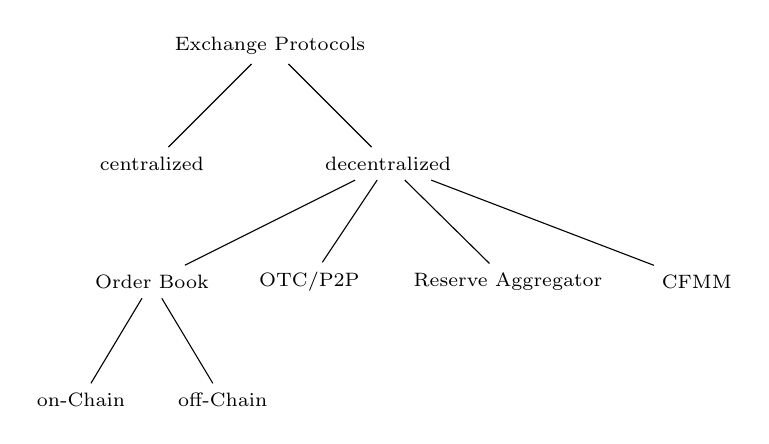
\begin{tikzpicture}
		[ sibling distance =10em ,
		every node/.style = {%shape=rectangle, rounded corners,
		%draw,
		font=\scriptsize,
		align = center,
		%top color=white, bottom color = highlight
		}]]
 		\tikzstyle{level 1}=[sibling distance=30mm]
 		\tikzstyle{level 2}=[sibling distance=20mm]
 		\tikzstyle{level 3}=[sibling distance=18mm]
  
  			\node {Exchange Protocols}
  			child { node {centralized}}
  			child { node {decentralized}
  				child { node {Order Book}
  					child { node {on-Chain}}
  					child { node {off-Chain}}}
  				child { node {OTC/P2P}}
  				child { node[right=-8mm] {Reserve Aggregator}}
  				child { node[right=1em] {CFMM}}
  			};
		\end{tikzpicture}
	\end{figure}
\end{frame}	
%%%


%%	
\begin{frame}{Why DEXs?}

	\textbf{Problems of CEXs:}
		\begin{small}
		\begin{itemize}
			\item A users' funds must be deposited with the exchange
			\item Access is forfeited and trust towards the exchange operator needed.
			\item Singe point of attack $\rightarrow$ Constant threat of becoming target of malicious third parties.
		\end{itemize}
		\end{small}	

\vspace{1.5em}

\uncover<2>{
	\textbf{Advantages of DEXs:}
		\begin{small}
		\begin{itemize}
			\item User remains in exclusive control of assets until trade is executed.
			\item Atomic trade execution = One indivisible transaction.
			\item No counterparty risk.
		\end{itemize}
		\end{small}
}
\end{frame}
%%%

%%%
\begin{frame}{The Emergence of Decentralized Exchanges}
Shapeshift V1:
\begin{itemize}
	\item Quote valid for 15 minutes
	\item Send token A to exchange address
	\item Get back token B immediately
	\item Not really decentralized
	\item Faced regulatory pressure
\end{itemize}
\vspace{0.5cm}

Etherdelta:
\begin{itemize}
	\item Onchain orderbook exchange %offchain orderbook?
	\item During ICO hype
	\item High fees
	\item Hacked
\end{itemize}

Constant Function Market Makers:
\begin{itemize}
	\item Currently highest volume
	\item Uniswap introduced in November 2018
\end{itemize}
\end{frame}
%%%

%%%
\begin{frame}{Constant Function Market Maker}

	\begin{figure}	
		\centering
		\begin{tikzpicture}
	
	% Pool
	\draw [thick] (-1,-1.5) -- (1,-1.5);
	\draw [thick](-1,-1.5) -- (-1, 0.6);
	\draw [thick](1,-1.5) -- (1, 0.6);
	\node [below=0.8cm] at (0,-0.8) {\scriptsize{Liquidity Pool}};
	
	% Balanced Pool
\uncover<2,3>{	
	\draw [fill=highlight] (-1,-1.5) rectangle (-0,0.25);
	\draw [fill=strongmint] (0,-1.5) rectangle (1,0.25);
}	

	% Unbalanced Pool
\uncover<4,5>{
	\draw [fill=highlight] (-1,-1.5) rectangle (-0,0);
	\draw [fill=strongmint] (0,-1.5) rectangle (1,0.5);
}	
\uncover<4>{
	\draw [dashed] (-1,0.25) -- (1,0.25);
}
	% Token labels
\uncover<2->{
\node at (-0.5,-0.7) {\scriptsize{CIF}};
\node at (0.5,-0.7) {\scriptsize{ETH}};
}

\uncover<4->{
 \node at (-4.5, 0.5) {\scriptsize{Pool Token}};
}
	
	%% LPs, Trader
	\uncover<1->{
		\node at (-4.5,-0.5) {\includegraphics[scale=0.03]{../assets/images/agents/agent_right}};
		\node at (-4,-0.8) {\includegraphics[scale=0.03]{../assets/images/agents/agent_right}};
		\node at (-5,-0.8) {\includegraphics[scale=0.03]{../assets/images/agents/agent_right}};
		\node [below=0.8cm] at (-4.5,-0.8) {\scriptsize{Liquidity Providers}};
		}
	\uncover<1->{
		\node at (4,-0.8) {\includegraphics[scale=0.05]{../assets/images/agents/agent_left}};
		\node [below=0.8cm]at (4,-0.8) {\scriptsize{Trader}};
		}
		
	%% Flow
	\uncover<2>{
		\draw[->] (-3.5, -0.8) -- (-1.5, -0.8) node [midway, below] {\includegraphics[scale=0.004]{../assets/images/eth}};
		\draw[->] (-3.5, -0.5) -- (-1.5, -0.5) node [midway, above]{\scriptsize{CIF}};
	}
	\uncover<3>{
	\draw[->] (-1.5, -0.8) -- (-3.5, -0.8) node [midway, above] {\scriptsize{Pool Token}};
	}
	\uncover<4>{
		\draw[->] (3.5, -0.8) -- (1.2, -0.8) node [midway, above] {\includegraphics[scale=0.004]{../assets/images/eth}};
		}

		
	\uncover<4>{
		\draw[->] (-0.5,0.12 ) arc (150:30:2.5cm) node [midway, above] {\scriptsize{CIF}};
	
		%\draw[dashed, <-] (-3.5,-2.5) arc (-130:-50:5.5cm) node [midway, above] {\scriptsize{Fees}};
	}
	
%	\uncover<5>{
%	\draw (0,1) node {\scriptsize{\textcolor{focus}{Arbitrage Opportunity}}};
%	\draw[-] (-0.25,0.8) -- (-0.25,0.25);
%	\draw[->] (-0.25,0.25) -- (0,0.25);
%	
%	}
		
	\end{tikzpicture}
	\end{figure}

\only<4>{
	\begin{itemize}
		\item The price is determined endogenously via a formula.
		\item The trader pays a fee which is added to the liquidity pool. Since no new Pool tokens are minted, this has the effect of splitting the transaction fee proportionally between all Liquidity Providers.
	\end{itemize}
}

\end{frame}
%%%


%%%
\begin{frame}{Arbitrage}
	\begin{figure}
		\begin{tikzpicture}
		
		\end{tikzpicture}
	\end{figure}
	\begin{itemize}
		\item When the pool price differs from the market price (e.g on a centralized exchange), there is an arbitrage opportunity. Therefore, the Pool Price should be the same as the Market Price.
	\end{itemize}	
\end{frame}
%%%


%%%
\begin{frame}{Constant Product Market Maker}
Constant Product Formula:
	\begin{align*}
		x \cdot y &= k
	\end{align*}

	\begin{itemize}
		\item[] x: amount of x-tokens in the pool
		\item[] y: amount of y-tokens in the pool
		\item[] k: constant
	\end{itemize}
	\vspace{1cm}
	\uncover<2->{
		Relative Prices are given by the first derivative of k:
		\vspace{0.2cm}
		\begin{itemize}
			\item[] $P_x = \frac{y}{x}$
			\item[] $P_y = \frac{x}{y}$
		\end{itemize}
	}
\end{frame}
%%%


%%%
\begin{frame}{Constant Product Market Maker}
	\begin{figure}[h!]
		\begin{center}
			\begin{tikzpicture}[]
    
    \draw[samples = 200, color=blue, scale=1, xshift = 0cm, yshift = 0cm, domain=0.9:4.55, smooth, variable=\x] plot ({\x}, {4/\x}) node[right,color=blue] {$k$} ;       
    
  	\draw[->] (0,0)--(5,0) node[below,midway]{} node[right] {$X$-tokens in liquidity pool} ;
    \draw[->] (0,0)--(0,5) node[above,midway,rotate=90]{} node[above] {$Y$-tokens in liquidity pool};  
  
    \draw[dotted, thick] (2,2)--(0,2) node[left]{\scriptsize $y$};

    \draw[dotted, thick] (2,2)--(2,0) node[below, yshift = -0.08cm]{\scriptsize $x$};
  
	\draw[fill=black] (2,2) circle(2pt);

\end{tikzpicture}
		\end{center}
	\end{figure}
\end{frame}
%%%


%%%
\begin{frame}{Constant Product Market Maker}
Constant Product Formula:
	\begin{align*}
		x \cdot y &= k
	\end{align*}
	
	\textbf{Properties:}
	\begin{itemize}
		\item<1-> Convexity of the indifference set
		\item<2-> Dynamic endogenous pricing model
		\item<3-> The pool will never be depleted and always be able to quote relative prices
	\end{itemize}
\end{frame}
%%%

%%%
\begin{frame}{Swap (without fees)}
	Let's assume a constant product market maker with no fees. Suppose an agent wants to exchange $\Delta x$ of x-tokens into y-tokens
	\vspace{0.5cm}
	\begin{figure}[h!]
		\begin{center}
			\begin{tikzpicture}
	
	% Pool
	\draw [thick] (-1,-1.5) -- (1,-1.5);
	\draw [thick](-1,-1.5) -- (-1, 0.6);
	\draw [thick](1,-1.5) -- (1, 0.6);
	\node [below=0.8cm] at (0,-0.8) {\scriptsize{Liquidity Pool}};
	
	% Balanced Pool
	\draw [fill=highlight] (-1,-1.5) rectangle (-0,0.25);
	\draw [fill=strongmint] (0,-1.5) rectangle (1,0.25);

	% Token labels
	\node at (-0.5,-0.7) {\scriptsize{y}};
	\node at (0.5,-0.7) {\scriptsize{x}};

	%% Trader
	\node at (4,-0.8) {\includegraphics[scale=0.05]{../assets/images/agents/agent_left}};
	\node [below=0.8cm]at (4,-0.8) {\scriptsize{Trader}};
		
	%% Flow
	\draw[->] (3.5, -0.8) -- (1.2, -0.8) node [midway, above] {\scriptsize{$\Delta x$}};
	\draw[->] (-0.5,0.12 ) arc (150:30:2.5cm) node [midway, above] {\scriptsize{$\Delta y$}};
		
\end{tikzpicture}
		\end{center}
	\end{figure}	
\end{frame}
%%%

%%%
\begin{frame}{Swap (without fees)}
	\begin{figure}[h!]
		\begin{center}
			\begin{tikzpicture}[]
    
    \draw[samples = 200, color=blue, scale=1, xshift = 0cm, yshift = 0cm, domain=0.9:4.55, smooth, variable=\x] plot ({\x}, {4/\x}) node[right,color=blue] {$k$} ;       
    
  	\draw[->] (0,0)--(5,0) node[below,midway]{} node[right] {$x$-tokens} ;
    \draw[->] (0,0)--(0,5) node[above,midway,rotate=90]{} node[above] {$y$-tokens};  
  
  	% Before Swap
    \draw[dotted, thick] (2,2)--(0,2) node[left]{\scriptsize $y$};
    \draw[dotted, thick] (2,2)--(2,0) node[below, yshift = -0.08cm]{\scriptsize $x$};
	\draw[fill=black] (2,2) circle(2pt);
	
	% After Swap
    \draw[dotted, thick] (3,1.333)--(0,1.333) node[left]{\scriptsize $y-\Delta(y)$};	
    \draw[dotted, thick] (3,1.333)--(3,0) node[below]{\scriptsize $x+\Delta(x)$};
	\draw[fill=black] (3,1.333) circle(2pt);

\end{tikzpicture}
		\end{center}
	\end{figure}
\end{frame}
%%%


%%%
\begin{frame}{Swap (without fees)}
	\vspace{0.5cm}
		\begin{align*}
			\onslide<1->{ y' &= \biggl( \frac{k}{x + \Delta x} \biggr) }\\
			\onslide<2->{ \Delta y &= y - \biggl( \frac{k}{x + \Delta x} \biggr) }\\
			\onslide<3->{ k' &= (x + \Delta x) \cdot (y - \Delta y) = k }
		\end{align*}	
\end{frame}
%%%


%%%
\begin{frame}{Swap (with fees)}
	Let us now assume a fee $\rho \in [0,1)$ with $\gamma = 1 - \rho$. The fee is charged on every trade and added to the liquidity pool and therefore leads to an increase in $k$. 
\end{frame}
%%%


%%%
\begin{frame}{Swap (with fees)}
	\begin{figure}[h!]
		\begin{center}
			\begin{tikzpicture}[]
    
 	\draw[->] (0,0)--(5,0) node[below,midway]{} node[right] {$x$-tokens} ;%{\small{$x$-tokens in liquidity pool}};
	\draw[->] (0,0)--(0,5) node[above,midway,rotate=90]{} node[above] {$y$-tokens};%{\small{$y$-tokens in liquidity pool}};

	% k before swap
 	\draw[samples = 200, color=blue, scale=1, xshift = 0cm, yshift = 0cm, domain=0.9:4.55, smooth, variable=\x] plot ({\x}, {4/\x}) node[right,color=blue] {$k$} ;    

	% k after swap
 	\draw[samples = 200, color=blue, scale=1, xshift = 0cm, yshift = 0cm, domain=1.345:4.55, smooth, variable=\x] plot ({\x}, {6/\x}) node[right,color=blue] {$k'$} ;    
	 
	% reserves before swap
	\draw[fill=black] (1.75,2.3) circle(2pt);
	\draw[dotted,thick] (1.75,2.3) -- (1.75,0) node[below]{\scriptsize{${x}$}};
	\draw[dotted,thick] (1.75,2.3) -- (0,2.3) node[left]{\scriptsize{$y$}};
	
	% reserves after swap (incl. fees)
	\draw[fill=black] (3.5,1.715) circle(2pt);
	\draw[dotted,thick] (3.5,1.715) -- (3.5,0) node[below]{\scriptsize{${x+\Delta(x)}$}};
	\draw[dotted,thick] (3.5,1.715) -- (0,1.715) node[left]{\scriptsize{${y-\Delta(y_\rho)}$}};
	
	% reserves after swap (excl. fees)
	\draw[dotted,thick] (3.5,1.13) -- (0,1.13) node[left]{\scriptsize{${y-\Delta(y_\rho)-\tau}$}};
 
\end{tikzpicture}
		\end{center}
	\end{figure}
\end{frame}
%%%

%%%
\begin{frame}{Swap (with fees)}
	\vspace{0.5cm}
		\begin{align*}
			\onslide<1->{ y'_\rho &= \biggl( \frac{k}{x + \gamma \cdot \Delta x} \biggr) }\\
			\onslide<2->{ \Delta y_\rho &= y - \biggl( \frac{k}{x + \gamma \cdot \Delta x} \biggr) }\\
			\onslide<3->{ k'_\rho &= (x + \Delta x) \cdot (y - \Delta y_\rho) > k }
		\end{align*}	
\end{frame}
%%%


%%%
\begin{frame}{Liquidity Provision}
Anyone can contribute liquidity to the pool, by providing $n$ $x$-tokens and $n \cdot \frac{y}{x}$ $y$-tokens to the smart contract.\\
	
	\begin{itemize}
		\item<2-> The liquidity provision only changes the token amounts and the constant $k$
		\item<3-> The ratio between the two tokens remains unchanged
		\item<4-> Both reserves are increased by the factor $\varphi = \frac{\Delta(x)}{x} = \frac{\Delta(y)}{y}$
	\end{itemize}

	\begin{align*}
		\onslide<5->{ x' &= x +\Delta x = (1+\varphi) x }\\
		\onslide<6->{ y' &= y +\Delta y = (1+\varphi) y}\\
		\onslide<7->{ k' &= (1+\varphi)^2 k	}
	\end{align*}
\end{frame}
%%%


%%%
\begin{frame}{Liquidity Provision}
	\begin{figure}[h!]
		\begin{center}
			\begin{tikzpicture}[]

	\draw[->] (0,0)--(5,0) node[below,midway]{} node[right] {\small{$X$-tokens in liquidity pool}} ;
	\draw[->] (0,0)--(0,5) node[above,midway,rotate=90]{} node[above] {\small{$Y$-tokens in liquidity pool}};
		
	% Before liquidity provision
	\draw[samples = 200, color=blue, scale=1, xshift = 0cm, yshift = 0cm, domain=0.9:4.55, smooth, variable=\x] plot ({\x}, {4/\x}) node[right,color=blue] {$k$};    
    \draw[dotted, thick] (2,2)--(2,0) node[below, yshift = -0.08cm]{\scriptsize $x$};
	\draw[dotted, thick] (2,2)--(0,2) node[left]{\scriptsize $y$};
	\draw[fill=black] (2,2) circle(2pt);

	% After liquidity provision
	\uncover<2->{
		\draw[->,dashed] (0,0)--(4.1,4.1);
	}
	\uncover<3->{
	    \draw[dotted, thick] (3,3)--(3,0) node[below]{\scriptsize $x'$};   
		\draw[->, red] (2.1, 0.1) -- (2.9, 0.1) node [midway, above] {\scriptsize{$\Delta x$}};
	}
	\uncover<4->{
    	\draw[dotted, thick] (3,3)--(0,3) node[left]{\scriptsize $y'$};
		\draw[fill=black] (3,3) circle(2pt);
		\draw[->, red] (0.1, 2.1) -- (0.1, 2.9) node [midway, right] {\scriptsize{$\Delta y$}};
		\draw[samples = 200, color=blue, scale=1, xshift = 0cm, yshift = 0cm, domain=2.025:4.55, smooth, variable=\x] plot ({\x}, {9/\x}) node[right,color=blue] {$k'$};  	
	}
\end{tikzpicture}
		\end{center}
	\end{figure}
\end{frame}
%%%


%%%
\begin{frame}{Divergence Loss}

	\textbf{General assumptions:} No fees, no other LPs \\ 
		\begin{enumerate}
			\item We provide 10 units both of ETH and CIF, which are equal in value ($1 \tfrac{CIF}{ETH}$).
			\begin{align*}
				10 \cdot 10 = 100	
			\end{align*}
			\item The price for ETH on the open market doubles, the price of CIF stays the same ($2 \tfrac{CIF}{ETH}$). After arbitrage, the pool balances should adjust to:
			\begin{align*}
				y &= \sqrt{k/P_{y}}	 = \sqrt{100/2} = 7.0716 \\
				x &= k / y = 100 / 7.0716 = 14.141
			\end{align*}
		\end{enumerate}	
\end{frame}
%%%


%%%
\begin{frame}{Divergence Loss}

	\begin{enumerate}
	\setcounter{enumi}{2}
		\item The total pool value, expressed in units of Token A is: 
			\begin{align*}
				7.0716 \cdot 2 \tfrac{CIF}{ETH} + 14.141 \cdot 1 \tfrac{CIF}{ETH} = 28.284 CIF
			\end{align*}
		\item If we simply held our initial allocation, we would have:
			\begin{align*}
			10 \cdot 2 \tfrac{CIF}{ETH} + 10 \cdot 1 \tfrac{CIF}{ETH} = 	30 CIF
			\end{align*}
		\item The difference between the Pool Value and the Hold Value is called divergence loss.
		\begin{align*}
			DL = \tfrac{Pool_V}{Hold_V} -1 = \tfrac{28.284}{30} - 1 = -5.72 \%
			\end{align*}
	\end{enumerate}	
	
	\begin{keytakeaway}{Note}
		In order to be profitable, a LP must collect more fees than the Divergence Loss. DL is only realized by selling the LP position (burning LP Tokens). There is no DL if the price ratio between the two pool assets stays equal.
	\end{keytakeaway}
	
\end{frame}
%%%


%%%
\begin{frame}{Swap one x-token with 0.03\% fee}
	%\textbf{Swap one x-token with a fee of 0.3 \%} \\ \vspace{1.5em}

	\begin{minipage}{0.5\textwidth}
		\begin{figure}[h!]
			\begin{center}
 				\begin{tikzpicture}[]
    
 	\draw[->] (0,0)--(5,0) node[below,midway]{} node[below, midway, yshift = -0.5cm] {\small{$X$-tokens in LP}};	
 	\draw[->] (0,0)--(0,5) node[above,midway,rotate=90]{} node[above] {\small{$Y$-tokens in LP}};

	% Initial reserves
 	\draw[samples = 200, color=blue, scale=1, xshift = 0cm, yshift = 0cm, domain=0.9:4.55, smooth, variable=\x] plot ({\x}, {4/\x}) node[right, below] {\scriptsize{$k$}} ;    
    \draw[dotted, thick] (2,2)--(0,2) node[left]{\scriptsize 10};
    \draw[dotted, thick] (2,2)--(2,0) node[below]{\scriptsize 10};
	\draw[red, fill=red] (2,2) circle(1.2pt);

	% Delta x
	\only<2>{
		\draw[->, red] (2.05, 0.1) -- (2.95, 0.1) node [midway, above] {\scriptsize{5}};	
	}
	\only<2 | handout:0>{
		\draw[dotted,thick] (3,1.3) -- (3,0) node[below]{\scriptsize{15}};	
	}
	\uncover<3-5>{
		\draw[dotted,thick] (3,1.3) -- (3,0) node[below]{};
	}
	
	% Delta x minus fees
	\uncover<3-4>{
		\draw[dotted, red, thick] (2.8,1.43) -- (2.8,0) node[below]{\scriptsize{14}};

	}
	\uncover<3-4>{
		\draw[->, red] (2.95, 0.625) -- (2.85, 0.625) node {};	
	}
	
	% y'
	\uncover<4 | handout:0>{	
		\draw[dotted,thick] (2.8,1.43) -- (0,1.43) node[left]{\scriptsize{$7.1429$}};
	}
	
	% k'
	\uncover<5->{
		\draw[samples = 200, color=blue, scale=1, xshift = 0cm, yshift = 0cm, domain=0.97:4.55, smooth, variable=\x] plot ({\x}, {4.3/\x}) node[right, above] {\scriptsize{$k'_\rho$}};

		\draw[dotted,thick] (3,1.43) -- (0,1.43) node[left]{\scriptsize{$7.1429$}};
		\draw[dotted, red, thick] (2.8,1.43) -- (2.8,0) node[below]{};
		\draw[red, fill=red] (3,1.43) circle(1.2pt);
		\draw[->, blue] (4.63, 0.85) -- (4.63, 1.0) node {};		
	}	
	\uncover<5- | handout:0>{
		\draw[dotted,thick] (3,1.3) -- (3,0) node[below]{\scriptsize{15}};	
	}
\end{tikzpicture}
			\end{center}
		\end{figure}
	\end{minipage}
\vspace{1em}
	\begin{minipage}{0.4\textwidth}
		\vspace{-4em}
		\begin{scriptsize}
			\begin{align*}
			\only<1>{
				\Delta y &= \dfrac{k}{x+ (1-\tau) \Delta x} - y \\
			}
			\only<2>{
			 	\Delta y &= \tfrac{100}{10+ (1-0.003) \cdot 10} - 10 = -0.9066 \\
		 		y' &= 10 - 0.9066 = 9.0934 \\
		 		k' &= 11 \cdot 9.0934 = 100.0274 \\
		 	}
		 	\only<3>{
		 		y' &= 10 - 0.9066 = 9.0934 \\
		 		k' &= 11 \cdot 9.0934 = 100.0274 \\
			}
			\only<4>{
				P &= \tfrac{y}{x} = \tfrac{10}{10} = 1 \\
				P_{swap} &= \tfrac{\Delta y}{\Delta x} = \tfrac{0.9066}{1} = 0.9066\\
				P' &= \tfrac{y'}{x'} = \tfrac{9.0934}{11} =  0.8267 \\
			}
			\only<5>{
				S &= \tfrac{Swap Price}{PR} - 1 = \tfrac{0.9066}{1} - 1 = -0.0934 \\
			}
			\end{align*}
		\end{scriptsize}
	\end{minipage}

\end{frame}
%%%


%%%
\begin{frame}{Swap one x-token in a bigger pool}
	%\textbf{Swap one x-token with a fee of 0.3 \%} \\

	\begin{minipage}{0.5\textwidth}
		\begin{figure}[h!]
			\begin{center}
				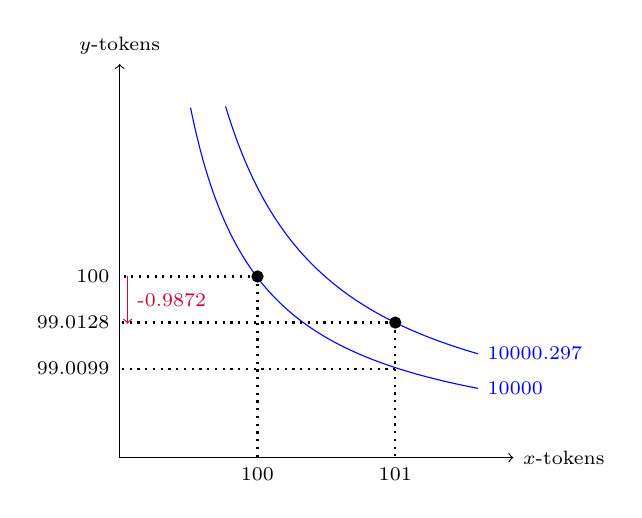
\begin{tikzpicture}[]
    
 	\draw[->] (0,0)--(5,0) node[below,midway]{} node[right] {\scriptsize{$x$-tokens}} ;%{\small{$x$-tokens in liquidity pool}};
	\draw[->] (0,0)--(0,5) node[above,midway,rotate=90]{} node[above] {\scriptsize{$y$-tokens}};%{\small{$y$-tokens in liquidity pool}};

	% k before swap
 	\draw[samples = 200, color=blue, scale=1, xshift = 0cm, yshift = 0cm, domain=0.9:4.55, smooth, variable=\x] plot ({\x}, {4/\x}) node[right,color=blue] {\scriptsize{10000}} ;    

	% k after swap
 	\draw[samples = 200, color=blue, scale=1, xshift = 0cm, yshift = 0cm, domain=1.345:4.55, smooth, variable=\x] plot ({\x}, {6/\x}) node[right,color=blue] {\scriptsize{10000.297}} ;    
	 
	% reserves before swap
	\draw[fill=black] (1.75,2.3) circle(2pt);
	\draw[dotted,thick] (1.75,2.3) -- (1.75,0) node[below]{\scriptsize{100}};
	\draw[dotted,thick] (1.75,2.3) -- (0,2.3) node[left]{\scriptsize{100}};
	
	% reserves after swap (incl. fees)
	\draw[fill=black] (3.5,1.715) circle(2pt);
	\draw[dotted,thick] (3.5,1.715) -- (3.5,0) node[below]{\scriptsize{101}};
	\draw[dotted,thick] (3.5,1.715) -- (0,1.715) node[left]{\scriptsize{99.0128}};
	\draw[->, red] (0.1, 2.3) -- (0.1, 1.7) node [midway, right] {\scriptsize{-0.9872}};
	
	% reserves after swap (excl. fees)
	\draw[dotted,thick] (3.5,1.13) -- (0,1.13) node[left]{\scriptsize{99.0099}};
 
\end{tikzpicture}
			\end{center}
		\end{figure}
	\end{minipage}
\vspace{1em}
	\begin{minipage}{0.4\textwidth}
		\vspace{-4em}
		\begin{scriptsize}
			\begin{align*}
			\only<1>{
				PR &= \tfrac{y}{x} = \tfrac{100}{100} = 1 \\
				P_{swap} &= \tfrac{\Delta y}{\Delta x} = \tfrac{0.9872}{1} = 0.9872\\
				PR' &= \tfrac{y'}{x'} = \tfrac{99.0128}{101} =  0.9803 \\
			}
			\only<2>{
				S &= \tfrac{P_{swap}}{P} - 1 = \tfrac{0.9872}{1} - 1 = -0.0128 \\
			}
			\end{align*}
		\end{scriptsize}
	\end{minipage}
	
	\uncover<2>{
	\begin{keytakeaway}{Impact of Pool/Trade Ratio}
	In our first example, the trader got 0.9066 y-Tokens, in the second 0.9872. When the trade size is smaller compared to the total pool liquidity, slippage is also reduced. In our example from $\approx$ 10\% to $\approx$ 1.3\%.
	\end{keytakeaway}

	}
		
\end{frame}
%%%



%%%
\begin{frame}{Other Bonding Curves}
	\begin{figure}
		\includegraphics[scale=0.6]{../assets/images/bonding-curves.png}
	\end{figure}
\end{frame}
%%%


%%%
\begin{frame}{Concentrated Liquidity}
	Concept of concentrated liquidity was first introduced in Uniswap V3 in March 2021\footnote{\href{https://uniswap.org/whitepaper-v3.pdf}{Uniswap V3 Whitepaper \link}}:
	\begin{itemize}
		\item<2-> Liquidity providers can add liquidity within a certain price range $[p_a, p_b]$.
		\item<3-> The position is active, if the price is within the given range.
		\item<4-> If the price is out of range, the liquidity provider only holds one asset and does not collect fees.
	\end{itemize}
	\vspace{0.5cm}
	\uncover<5->{
	\begin{keytakeaway}{Implications of Concentrated Liquidity}
		\begin{itemize}
			\item<5-> Higher capital efficiency
			\item<6-> Liquidity providers with concentrated liquidity earn more fees
			\item<7-> But: higher divergence loss risk
		\end{itemize}
	\end{keytakeaway}

	}
\end{frame}
%%%


%%%
\begin{frame}{Concentrated Liquidity}
	\begin{figure}[h!]
		\begin{center}
			\begin{tikzpicture}[]

	\draw[->] (0,0)--(5,0) node[below,midway]{} node[right] {\small{Price}} ;
	\draw[->] (0,0)--(0,5) node[above,midway,rotate=90]{} node[above] {\small{Liquidity}};

	% V2
	\only<1>{
		\draw [fill=highlight] (0,0) rectangle ++(5,1);
		\node [below] at (0,0) {\scriptsize{0}};
		\node [below] at (5,0) {\scriptsize{$\infty$}};
	}
	% Single position
	\only<2>{
		\draw [fill=strongmint] (1.5,0) rectangle ++(2,1.5);
		\node [below] at (1.5,0) {\scriptsize{$P_a$}};
		\node [below] at (3.5,0) {\scriptsize{$P_b$}};
	}
	
	% Multiple positions
	\only<3>{
		\draw [fill=highlight] (0,0) rectangle ++(5,1);
		\draw [fill=strongmint] (1.5,1) rectangle ++(2,1.5);
		\node [below] at (1.5,0) {\scriptsize{$P_a$}};
		\node [below] at (3.5,0) {\scriptsize{$P_b$}};
	}	
	
\end{tikzpicture}
		\end{center}
	\end{figure}	
\end{frame}
%%%


%%%
\begin{frame}{More than two Pool Assets}
\begin{itemize}
	\item The constant of UniSwap can also be extended to pools with more than two assets.
	\item Constant Mean Formula:
		\begin{align*}
			V = \prod_t B^{w_{t}}_{t}
		\end{align*}
	V : constant, w : normalized weight $[0,1]$, B : Balance
	\item The Constant Product formula is basically just a subset of the Constant Mean formula with two equally weighted assets ($w_t$ = 0.5).
\end{itemize}

\end{frame}
%%%


%%%
\begin{frame}{Concept of Aggregators}

\begin{figure}[t]
	\centering	
	\resizebox{0.8\textwidth}{!}{
	\begin{tikzpicture}[scale=1.0, every node/.style={scale=1.0}]
			\input{../assets/figures/defi_stack.tex}
	\end{tikzpicture}}
	\caption{The DeFi Stack \cite{FS:21}}
\end{figure}
\vspace{-1em}
\begin{itemize}
	\item DEX Aggregators source liquidity from different DEXs
	\item They allow a user to compare different swap prices and to choose on which DEX their trade is performed.
\end{itemize}


%DEX aggregators source liquidity from different DEXs and thus offer users better token swap rates than they could get on any single DEX. DEX aggregators have the ability to optimize slippage, swap fees and token prices which, when done right, offer a better rate for users.
\end{frame}
%%%


%%%
\begin{frame}{Frontrunning}

\end{frame}
%%%


%%%
\begin{frame}{Add. Liquidity Mining \& Vampire Attack}

\end{frame}
%%%


%%%
\begin{frame}{Initial DEX offerings}

\end{frame}
%%%


%%%
\begin{frame}{Exercise}
	\begin{exercise}{Exercise 1}
	For this exercise we use the ERC20 Token created in one of the previous videos (select Ropsten). Go to UniSwap Frontend Link to complete the following tasks:
	
		\begin{enumerate}
			\item Swap ETH to CIF
			\item Provide liquidity to ETH/CIF Pool
			\item Make another Swap
			\item Remove your liquidity position and analyze what happened
		\end{enumerate}
	\end{exercise}
\end{frame}
%%%



%%%
\begin{frame}%[allowframebreaks]
\frametitle{References and Recommended Reading}
	% Uniswap Whitepaper
	% Curve Whitepaper
	\bibliographystyle{amsplain}
	\bibliography{../assets/bib/refs}
\end{frame}
%%%





\end{document}